\documentclass{article}
\usepackage[utf8]{inputenc}
\usepackage{graphicx}

\title{\textbf{IF689 - Informática Teórica}}
\author{Aline Kessy Maciel de Oliveira}
\date{Outubro 2020}

\begin{document}

\maketitle
\begin{figure}[htb]
    \centering
    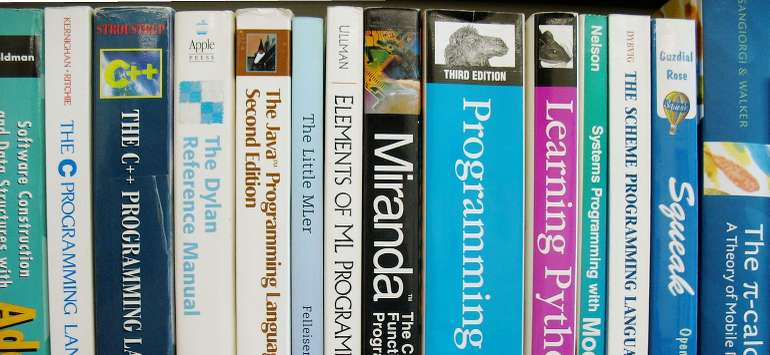
\includegraphics[scale=0.3]{imagem/livros.jpg}
    \caption{Livros de Informática [1]}
    \label{fig:my_label}
\end{figure}

\section{Introdução}

\par A disciplina de Informática Teórica aborda os conceitos da teoria da computação, e busca determinar quais problemas podem ser computados em um dado modelo de computação. Estuda os problemas computacionais e as classes das linguagens que podem ser produzidas e reconhecidas por modelos computacionais simbólicos. Também estuda a complexidade dos algoritmos.[2]

\section{Desenvolvimento}
\par Se trata de saber a noção do procedimento efetivo, que deu origem às primeiras "máquinas abstratas de computação efetiva" (como, por exemplo, a chamada Máquina de Turing, o primeiro modelo de computador programável por software, e que deu origem à chamada Tese de Church que afirma que qualquer função efetivamente computável pode ser computável por uma Máquina de Turing apropriadamente definida) está intimamente ligada à noção de "dedução em um sistema formal (simbólico)", como concebido por Gottlob Frege, o mentor da Lógica Moderna, justamente porque esta última veio como a implementação do sonho do filósofo Leibniz (século XVII) de criar uma máquina de verificação da validade de argumentos. [3]

\section{Relevância}
\par Em sua ementa, mostra a relevância em aprender a introdução, análise de algoritmos, complexidade computacional e computabilidade.

\section{Relação com outras disciplinas}
A disciplina Informática Teórica possui outras disciplinas como pré-requisito, dentre elas, são:

    
\begin{itemize}
\item  IF672 - Algorítmos e Estruturas de Dados
\item  IF673 - Lógica para Computação
\end{itemize}

    
    
\section{Referências}

\begin{itemize}
\item [1] EDITORIAL. Programação por computador: +500 livros gratuitos. Site: Coordinamento NetWorkers.

\item [2] Informática Teórica - CInWiki - CIn-UFPE.

\item [3] Site oficial da disciplina. Informática Teórica (IF689) - CIn-UFPE.
\end{itemize}

\end{document}